\documentclass{standalone}
\usepackage{libertine}
\usepackage[dvipsnames]{xcolor}
\usepackage{tikz}
%\usepackage{fix-cm}
\definecolor{color2}{HTML}{1F77B4}
\definecolor{color1}{HTML}{FF7F0E}
\setlength{\parskip}{0pt}
\setlength{\baselineskip}{0pt}
%\usetikzlibrary{fit}
\usetikzlibrary{calc}
\usetikzlibrary{decorations.markings}
\usetikzlibrary{decorations.shapes}
\usetikzlibrary{decorations.pathreplacing}
\usetikzlibrary{intersections}
\usetikzlibrary{patterns}
\tikzset{%
  from end of path/.style={
    insert path={
      \pgfextra{%
        \expandafter\pgfprocesspathextractpoints%
          \csname tikz@intersect@path@name@#1\endcsname%
        \pgfpointlastonpath%
        \pgfgetlastxy\lastx\lasty
      }
      (\lastx,\lasty)
}}}
%\tikzset{-dot-/.style={decoration={
%  markings,
%  mark=at position #1 with {\fill[color=red] circle (0.5mm);}},postaction={decorate}}}  
\tikzset{-dot3-/.style n args={2}{decoration={
  markings,
  mark=at position #1 with {\draw[-](0.0,-0.025) -- (0,0.025);\node[align=center,font=\fontsize{1mm}{0}\selectfont,inner sep=0mm] at (0, -0.05) {#2};}},postaction={decorate}}}

    \tikzset{
        hatch distance/.store in=\hatchdistance,
        hatch distance=10pt,
        hatch thickness/.store in=\hatchthickness,
        hatch thickness=2pt
    }

\newcommand{\barwidth}{0.5}
\newcommand{\barheight}{0.175} 

\begin{document}
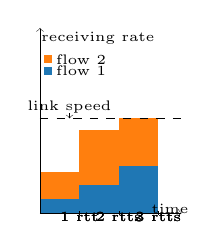
\begin{tikzpicture}
    
    \makeatletter
    \pgfdeclarepatternformonly[\hatchdistance,\hatchthickness]{flexible hatch}
    {\pgfqpoint{0pt}{0pt}}
    {\pgfqpoint{\hatchdistance}{\hatchdistance}}
    {\pgfpoint{\hatchdistance-1pt}{\hatchdistance-1pt}}%
    {
        \pgfsetcolor{\tikz@pattern@color}
        \pgfsetlinewidth{\hatchthickness}
        \pgfpathmoveto{\pgfqpoint{0pt}{0pt}}
        \pgfpathlineto{\pgfqpoint{\hatchdistance}{\hatchdistance}}
        \pgfusepath{stroke}
    }
    \makeatother
 
%\draw[dashed] (0,1) -- ++(2.5,0);
%\node[align=center,font=\fontsize{3pt}{0}\selectfont,inner sep=0mm] at (2.25, 0.75) (bufferSizeLabel) {BDP+\\ buffer size};
%\draw[->, line width=0.05mm] (bufferSizeLabel) -- (2.25,1);
%\draw[name path=A] (0,0.5)-- ++(0.5, 0.5);
%\draw[from end of path=A, name path=B, -dot-=0, -dot-=0.5, -dot-=1] -- ++(0.25,0);
%\node[align=center,font=\fontsize{3pt}{0}\selectfont,inner sep=0mm] at (0.5, 0.7) (lossLabel) {packet loss};
%\draw[->, line width=0.05mm] (lossLabel) -- (0.5,0.95);
%\draw[from end of path=B, name path=C] ++(0,-0.5mm) -- ++(0,-0.95cm) -- ++(1,1);
%\draw[from end of path=C, name path=D, -dot-=0, -dot-=0.5, -dot-=1] -- ++(0.25,0);
%\draw[from end of path=D, name path=E] ++(0,-0.5mm) -- ++(0,-0.95cm) -- ++(0.5,0.5);


%\draw[draw,decorate,decoration={brace, mirror}] (2.5,0) -- ++(0.0,1) node [midway,right,align=left,font=\fontsize{3pt}{0}\selectfont] {buffer\\ size};
%
%\draw[dashed] (0,0) -- ++(2.5,0);
%\node[align=center,font=\fontsize{3pt}{0}\selectfont,inner sep=0mm] at (1.95,-0.25) (optimal) {optimal minimum\\ window (BDP)};
%\draw[->, line width=0.05mm] (optimal) -- ++(0,0.25);

\node at (\barwidth /2, \barheight /2) [inner sep=0,fill=color2,rectangle,minimum width=\barwidth cm,minimum height=\barheight cm] {};
\node at (\barwidth /2, 2*\barheight) [inner sep=0,fill=color1,rectangle,minimum width=\barwidth cm,minimum height=2*\barheight cm] {};

\node at (\barwidth /2 + \barwidth, \barheight) [inner sep=0,fill=color2,rectangle,minimum width=\barwidth cm,minimum height=2*
\barheight cm] {};
\node at (\barwidth /2 + \barwidth, 4*\barheight) [inner sep=0,fill=color1,rectangle,minimum width=\barwidth cm,minimum height=4*\barheight cm] {};

\node at (\barwidth /2 + 2*\barwidth, 0.3) [inner sep=0,fill=color2,rectangle,minimum width=\barwidth cm,minimum height=0.6cm] {};
\node at (\barwidth /2 + 2*\barwidth, 0.9) [inner sep=0,fill=color1,rectangle,minimum width=\barwidth cm,minimum height=0.6cm] {};

\draw[dashed] (0,1.2) -- ++(1.8,0);
\node[align=center,font=\fontsize{2.75pt}{0}\selectfont,inner sep=0mm] at (0.375, 1.35) (maximum) {link speed};
\draw[->, line width=0.05mm] (maximum) -- (0.375,1.2);

\node[anchor=north west, align=center,font=\fontsize{3pt}{0}\selectfont,inner sep=0mm] at (0.01, 2.3) (rate) {receiving rate};

%\draw[draw,decorate,decoration={brace,mirror}] (0.75,0) -- (1.75,0) node [inner sep=0, outer sep=0,midway,below,yshift=-1.25mm,font=\fontsize{3pt}{0}\selectfont] {interval};
%\draw[densely dotted] (1.75,0) -- (1.75,0.95);

\newcommand{\xaxislength}{1.8}

\draw[->, line width=0.05mm, -dot3-={0.5 cm}{1 rtt}, -dot3-={1.0 cm}{2 rtts}, -dot3-={1.5 cm}{3 rtts}] (0,0) -- ++(\xaxislength , 0);
\node[align=center,font=\fontsize{3pt}{0}\selectfont,inner sep=0mm] at (1.65, 0.05) (time) {time};

\draw[->, line width=0.05mm] (0,0) -- ++(0,2.35);
\draw[draw=none, line width=0.05mm] (-0.05,-0.0) -- ++(0,1);
\draw[draw=none, line width=0.05mm] (0,-0.05) -- ++(0,1);

\node (red_label) at (0.1,1.95) [inner sep=0,fill=color1,rectangle,minimum width=0.1cm,minimum height=0.1cm,label={[align=left,label distance=-0.75mm]right:\fontsize{1mm}{0mm}\selectfont{}flow 2}] {};

\node (green_label) at (0.1,1.8) [inner sep=0,fill=color2,rectangle,minimum width=0.1cm,minimum height=0.1cm,label={[align=left,label distance=-0.75mm]right:\fontsize{1mm}{0mm}\selectfont{}flow 1}] {};

\end{tikzpicture}
\end{document}
